%==============================================================================
% results.tex — Results for PP-HFM
% Self-contained \section{}; \input this into main.tex (never compile alone).
%
% STATUS: partial. Only subsections whose experiments are COMPLETE and whose
% numbers are read from a results artifact appear here. Pending subsections are
% listed at the end of this file as comments, each naming the experiment and
% the artifact that will supply it. Do not write a number into this file that
% does not appear in a file under SIMULATORS/results/.
%
% Every figure quoted below is traceable:
%   objectives_vitaldb.json   O1, O1b, O2a, O2b, O3a, O3b, O4
%   objectives_wear.json      same, wearable deployment
%   latency_*.json            per-stage latency decomposition
%   ns3_results_*.csv         round latency, reliability (all rows packet-level)
%   cloudsim_results_*.csv    per-tier energy
%==============================================================================

\section{Results}
\label{sec:results}

\subsection{System-Level Objectives}
\label{sec:results:objectives}

The framework is evaluated on two deployments that differ in client
composition. In the clinical deployment, nine institutional clients hold the
records of $6{,}257$ patients, so each client contains many individuals, and
each individual contributes $7.8$ records on average. In the wearable
deployment, each of the twenty-two clients corresponds to a single participant
who contributes approximately $1{,}750$ records. The second deployment also
tests whether the system-level behavior generalizes across topology and payload
size.

Table~\ref{tab:results_objectives} reports the measured value of each design
objective of Table~\ref{tab:objectives}. All targets are met on the clinical
deployment. On the wearable deployment, all targets are met except the accuracy
bound, which is inconclusive.

\begin{table}[!t]
\centering
\caption{Measured outcomes against the pre-registered targets of
Table~\ref{tab:objectives}. Network quantities are measured at packet level on
every simulated round of both deployments. The accuracy row is a paired
comparison against a non-private reference trained under the identical recipe;
$^{\dagger}$ marks an interval that spans its threshold and is therefore
inconclusive at the pre-registered sample size.}
\label{tab:results_objectives}
\small
\setlength{\tabcolsep}{4pt}
\begin{tabular}{llrrl}
\toprule
& Quantity & Clinical & Wearable & Target \\
\midrule
O1  & Uplink reduction   & $90.8\%$   & $96.1\%$   & $\ge 50\%$ \\
O1b & Round latency      & $16.9\%$   & $21.7\%$   & improvement \\
O2a & Budget (composed)  & $0.970$    & $0.966$    & $\varepsilon \le 1$ \\
O2b & Accuracy change    & $-0.92$ pp & $1.97^{\dagger}$ pp & $\le 2$ pp \\
O3a & Latency (P95)      & $4.58$ ms  & $1.22$ ms  & $< 100$ ms \\
O3b & Update success     & $100.00\%$ & $99.94\%$  & $> 99\%$ \\
O4  & Energy saving      & $72.3\%$   & $76.8\%$   & $\ge 20\%$ \\
\bottomrule
\end{tabular}
\end{table}

\begin{table}[!t]
\centering
% !! STALE: latency_vitaldb.json (2026-09-06) gives total mean 2.912 / P95 3.048 ms
% !! on the FP32 graph, 200 runs. Values and caption below are from an older run.
% !! Resolve before submission (see session notes 2026-10-21).
\caption{Inference latency decomposition, integer-quantized graph on a CPU
provider, 1000 timed executions after 100 discarded warm-up executions.}
\label{tab:latency}
\begin{tabular}{lrr}
\toprule
Stage & Mean (ms) & P95 (ms) \\
\midrule
Preprocessing              & 0.140 & 0.147 \\
Forward pass               & 4.221 & 4.395 \\
Conformal set construction & 0.030 & 0.037 \\
Post-processing            & 0.011 & 0.014 \\
\midrule
Total                      & 4.401 & 4.582 \\
\bottomrule
\end{tabular}
\end{table}

\begin{figure*}[!t]
\centering
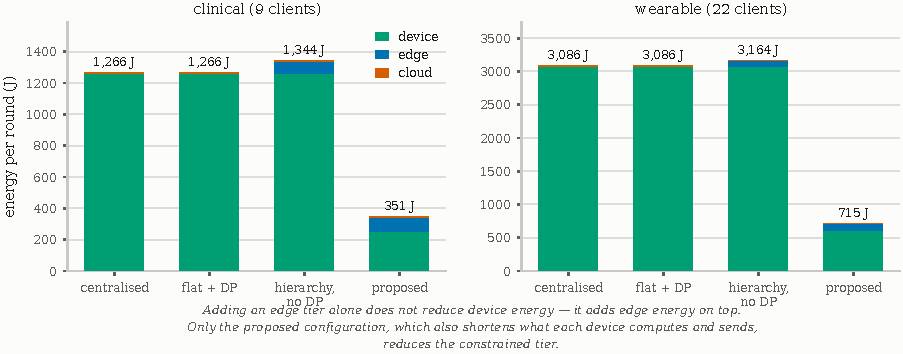
\includegraphics[width=\textwidth]{fig7_energy.pdf}
\caption{Energy per training round, attributed by tier, on both deployments.
The hierarchy alone redistributes work without reducing it: device energy is
unchanged and edge energy is added. Only the proposed configuration reduces the
energy of the constrained tier.}
\label{fig:energy}
\end{figure*}

All network quantities are measured on every simulated round. An earlier
simulator configuration evaluated one round in ten at packet level and composed
the remaining rounds analytically. The two approaches disagree: the analytical
model placed the communication term of the centralized baseline at $256$ ms,
whereas the simulated network delivers $23.6$ ms, which overstated the latency
benefit of the hierarchy by a factor of about four. No analytically composed
rounds contribute to the values reported here.

The reported privacy budget is the composed total. Training accounts for
$\varepsilon = 0.7705$ and the release of the conformal calibration quantile
for a further $0.2000$, giving $0.970$ against a budget of one. Reporting only
the training term would understate the expenditure by $23\,\%$.

\subsubsection{Communication and latency}
Two-tier aggregation reduces uplink traffic by $90.8\,\%$ relative to
centralized training, against a target of $50\,\%$. The measurement is taken
from the deployed compressor and includes the index array that top-$\kappa$
sparsification transmits with the retained values, which analytical payload
estimates omit and which is not negligible at high sparsity.

The hierarchy also reduces the end-to-end latency of a training round from
$90.5$ ms to $75.2$ ms in the clinical deployment, a reduction of $16.9\,\%$.
The reduction is positive in every simulated round, ranging from $8.2\,\%$ to
$25.8\,\%$. It is smaller than the traffic reduction because the communication
term falls from $23.6$ ms to $16.5$ ms, while the compute terms (sensing,
preprocessing, inference and aggregation) are common to all topologies and
dominate the total. The hierarchy reduces link time, not computation.

In the wearable deployment, round latency falls from $104.5$ ms to $81.8$ ms,
or $21.7\,\%$, with the communication term falling from $37.6$ ms to
$23.2$ ms. The larger reduction is consistent with the larger topology:
twenty-two stations contend for the same wireless medium rather than nine, so
uplink latency is a larger share of the total. The latency benefit of the
hierarchy therefore depends on the topology.

\subsubsection{Cost of a valid guarantee}
The results above were obtained with the oracle encoder configuration, in which
the frozen representation was pretrained on the pooled client training data.
This configuration does not provide a valid end-to-end guarantee, and its
utility is therefore an upper bound. With the disjoint configuration, in which
the encoders are pretrained only on a population reserved before federated
training and disjoint from every client, the area under the ROC curve decreases
by $0.0322$ $(0.8429 \rightarrow 0.8107)$, by $0.0310$ at the case level, and
average precision by $0.0763$. This difference is the cost of an end-to-end
valid guarantee. Comparisons between arms are unaffected, because all arms
share the same encoders.

\subsubsection{Privacy and utility}
The composed budget of $0.970$ satisfies the requirement $\varepsilon \le 1$.
Relative to a non-private reference trained with the same recipe, the change in
balanced accuracy is $-0.92$ pp, with a paired $95\,\%$ confidence interval of
$[-2.82, +0.99]$ over five seeds. The interval contains zero, so no accuracy
cost is detectable at this sample size. The requirement of at most $2$ pp is
met.

On the wearable deployment, the same comparison gives $1.967$ pp with an
interval of $[1.760, 2.173]$ over fifteen seeds. The interval spans the $2$ pp
threshold, so this objective is \emph{inconclusive}. The seed count was fixed
in advance and was not increased after inspecting the interval.

\subsubsection{Quality of service}
Table~\ref{tab:latency} decomposes the inference latency. Construction of the
conformal prediction set, which provides the coverage guarantee, takes
$0.030$ ms of the $4.401$ ms mean inference time, or $0.68\,\%$, and $0.037$ ms
at the $95$th percentile. The differentially private mechanism adds no
inference cost, because its noise is applied to gradients during training and
changes only the parameter values. The conformal set is therefore the only
guarantee-related component with an inference cost, at less than one percent
of the total.

The 95th-percentile latency is $4.58$ ms in the clinical deployment and
$1.22$ ms in the wearable deployment, against a budget of $100$ ms, both
measured on the integer-quantized graph on a CPU provider. This twentyfold
margin is due to the compact fusion head and integer arithmetic, not to the
hierarchy or the privacy mechanism. The difference between the deployments
follows from the input dimension. The margin allows a larger backbone to be
used within the same latency budget.

Update delivery succeeds for $100.00\,\%$ of transmissions in the clinical
deployment and $99.94\,\%$ in the wearable deployment, against a target of
$99\,\%$. Both values are measured on every round. Under the earlier
configuration, in which nine rounds in ten were composed analytically, the
clinical value was $99.27\,\%$. The wearable deployment does not reach perfect
delivery, with a per-round minimum of $99.15\,\%$, as expected when twenty-two
stations share one medium.

\subsubsection{Energy}
Energy per round decreases from $1266.2$ J to $350.8$ J in the clinical
deployment, a saving of $72.3\,\%$, and from $3086.2$ J to $714.8$ J in the
wearable deployment, a saving of $76.8\,\%$, against a target of $20\,\%$.
Energy is reported per tier because a hierarchy redistributes computation
rather than eliminating it (Fig.~\ref{fig:energy}). Introducing the edge tier
\emph{alone} leaves device energy unchanged and adds edge energy, so the total
increases from $1266$ J to $1344$ J. The saving occurs only in the configuration
that also reduces device-side computation and transmission, which lowers the
device term fivefold.

\subsection{The Privacy Unit and the Budget}
\label{sec:results:unit}

Two comparisons quantify the cost of the design decisions of
Section~\ref{sec:method:privacy}. Both are paired by seed against an arm that
differs only in the factor under test.

\subsubsection{Cost of moving the unit from the record to the individual}
Enforcing the guarantee over individuals rather than records reduces the area
under the ROC curve by $0.0188$, with a paired $95\,\%$ interval of
$[-0.0255, -0.0120]$ over five seeds. The case-level change is $-0.0193$
$[-0.0266, -0.0120]$, and average precision decreases by $0.0783$
$[-0.1046, -0.0520]$. These intervals exclude zero. The cost is larger in
average precision than in the area under the ROC curve, consistent with the
minority class being harder to fit under a coarser sampling unit.

Two effects contribute to this cost. Sampling patients rather than records
reduces the number of effective units per step from $34{,}044$ to $4{,}372$ on
this partition, and clipping a patient's summed gradient constrains
individuals with many records more strongly than those with few.
Section~\ref{sec:results:kscaling} isolates the second effect by holding the
number of units per step equal in both arms.

\subsubsection{Initialization, not the privatized subset}
The proposed recipe differs from conventional private training in two
respects: it starts from pretrained encoders, and it privatizes only the
fusion head. A two-arm comparison cannot separate these factors, so three arms
are compared. B4 is full-model private training from a random initialization,
the prior-art configuration. B7 is full-model private training from the
pretrained initialization, which changes only the initialization. B6 is
head-only private training from the pretrained initialization, which changes
only the privatized subset. Fig.~\ref{fig:epsilon} shows the three arms on the
clinical corpus, and Table~\ref{tab:recipe} reports both steps on both
deployments over three seeds.

\begin{table}[!t]
\centering
\caption{Decomposition of the recipe in macro AUROC, three seeds. The
initialization step B4$\rightarrow$B7 holds the privatized subset at the whole
network and changes only the starting point; the subset step
B7$\rightarrow$B6 holds the starting point and privatizes $30\,\%$ of the
network instead of all of it, and is reported as mean $\pm$ a Student-$t$
half-width because it is the step the claim turns on.}
\label{tab:recipe}
\setlength{\tabcolsep}{3.5pt}
\small
\begin{tabular}{lcccc}
\toprule
& \multicolumn{2}{c}{Clinical} & \multicolumn{2}{c}{Wearable} \\
\cmidrule(lr){2-3}\cmidrule(lr){4-5}
$\varepsilon$ & B4$\rightarrow$B7 & B7$\rightarrow$B6 & B4$\rightarrow$B7 & B7$\rightarrow$B6 \\
\midrule
$\infty$ & $+0.0187$ & $+0.0036 \pm 0.0329$ & $+0.0021$ & $-0.0002 \pm 0.0003$ \\
$8$      & $+0.0649$ & $+0.0014 \pm 0.0084$ & $+0.0883$ & $+0.0001 \pm 0.0002$ \\
$4$      & $+0.0803$ & $+0.0033 \pm 0.0049$ & $+0.1257$ & $+0.0001 \pm 0.0002$ \\
$2$      & $+0.0985$ & $+0.0031 \pm 0.0063$ & $+0.1918$ & $+0.0002 \pm 0.0001$ \\
$1$      & $+0.1221$ & $+0.0026 \pm 0.0122$ & $+0.2827$ & $+0.0003 \pm 0.0008$ \\
$0.5$    & $+0.1447$ & $+0.0030 \pm 0.0204$ & $+0.3580$ & $+0.0013 \pm 0.0088$ \\
\bottomrule
\end{tabular}
\end{table}

Almost the entire effect is due to the initialization, and it increases as the
budget tightens. On the clinical corpus, the change from random to pretrained
initialization is worth $0.0187$ without noise and $0.1447$ at the tightest
budget, increasing monotonically in between; on the wearable corpus it ranges
from $0.0021$ to $0.3580$. Restricting the privatized subset is worth at most
$0.0036$ on the clinical corpus and $0.0013$ on the wearable corpus at any
budget, and its intervals cover zero throughout.

This result contradicts a dimensionality explanation. If the advantage arose
because a smaller parameter vector absorbs less noise, B7, which privatizes all
$1{,}864{,}227$ parameters, should perform worse than B6, which privatizes
$559{,}874$, and the difference should be largest at the tightest budget. At
$\varepsilon = 0.5$, however, the two arms differ by only $0.0030$, with an
interval covering zero, although B7 privatizes $3.3$ times as many parameters
under the same budget. This is consistent with the noise scale being determined
by the budget, the number of steps and the sampling rate rather than by the
number of parameters.

The same pattern appears in sensitivity to the budget. Across the full range,
the randomly initialized arm loses $0.1181$ on the clinical corpus and $0.3716$
on the wearable corpus, where it falls to $0.6247$, close to chance. Both
pretrained arms change by less than $0.016$ on either deployment. Robustness to
a tight budget is therefore determined by the initialization. Under a fixed
budget, a legitimate pretrained initialization should take priority over the
choice of privatized parameters.

Restricting the privatized subset does reduce communication. Only head
parameters are transmitted, which produces the uplink reductions reported in
Section~\ref{sec:results:objectives}, and Table~\ref{tab:recipe} shows that this
comes at no measurable cost in accuracy. It is not, however, an accuracy
mechanism, and a two-arm comparison of head-only training from a pretrained
initialization against full-model training from a random initialization does
not support such a claim, because the two arms differ in both respects.

\begin{figure}[!t]
\centering
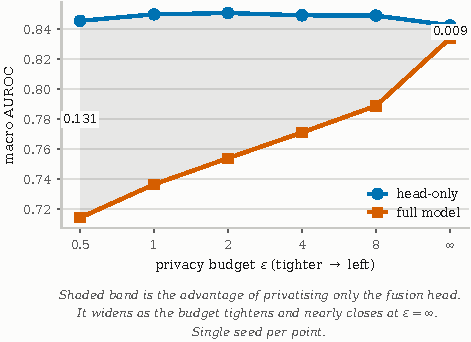
\includegraphics[width=\columnwidth]{fig8_epsilon.pdf}
\caption{Decomposing the recipe across the budget on the clinical corpus. The
shaded band is the initialization effect, obtained with the privatized subset
held at the whole network, and it is nearly the entire advantage. The two
pretrained arms nearly coincide at every budget, although one privatizes $3.3$
times as many parameters as the other, which excludes an explanation based on
privatized dimensionality. Three seeds per point.}
\label{fig:epsilon}
\end{figure}

\subsubsection{Records per individual}
\label{sec:results:kscaling}
Because a patient-level guarantee bounds the \emph{summed} contribution of an
individual, its cost is expected to increase with the number of records per
individual and to vanish when each individual contributes a single record.
Table~\ref{tab:kscaling} reports both arms as $k$, the number of training
records retained per patient, is varied over $\{1, 2, 4, 8\}$ with three seeds.
The number of units sampled per step is equal in both arms, which removes the
sampling-rate effect, so only the clipping geometry differs. The validation and
test partitions are unchanged.

\begin{table}[!t]
\centering
\caption{Average precision by records per individual $k$. The gap is paired by
seed and reported as mean $\pm$ the half-width of a Student-$t$ interval over
three seeds; an interval excluding zero is one whose half-width is smaller than
its mean.}
\label{tab:kscaling}
\setlength{\tabcolsep}{4pt}
\begin{tabular}{ccccc}
\toprule
$k$ & Record & Individual & Gap & $p$ \\
\midrule
$1$ & $0.5015$ & $0.5067$ & $-0.0052 \pm 0.0613$ & $0.7514$ \\
$2$ & $0.5590$ & $0.5084$ & $0.0507 \pm 0.0090$ & $0.0017$ \\
$4$ & $0.5924$ & $0.5092$ & $0.0832 \pm 0.0138$ & $0.0015$ \\
$8$ & $0.5955$ & $0.5089$ & $0.0866 \pm 0.0263$ & $0.0049$ \\
\bottomrule
\end{tabular}
\end{table}

At $k = 1$, the two arms are indistinguishable, with a gap of $-0.0052$ and an
interval covering zero, as required by the construction. The divergence at
larger $k$ can therefore be attributed to the privacy unit rather than to the
experimental setup. From $k = 2$ onward, the gap is resolved and increases
monotonically, reaching $0.0866$ at $k = 8$; the increment from $k = 4$ to
$k = 8$ is an order of magnitude smaller than the preceding one.

The individual-level arm remains flat in $k$, within $[0.4967, 0.5176]$ across
all configurations, whereas the record-level arm increases from $0.5015$ to
$0.5955$. The widening gap therefore reflects a lack of improvement under the
stricter unit rather than a degradation. Additional records per patient provide
signal that the record-level arm exploits and the individual-level arm cannot,
because the bound on the summed contribution is tightest for the individuals
who contribute the additional records. On this corpus, collecting more data per
patient therefore increases the relative cost of an individual-level guarantee.

The area under the ROC curve changes in the same direction, by $0.0006$,
$0.0094$, $0.0133$ and $0.0132$ over the same values of $k$, but every interval
covers zero at three seeds. The effect is therefore resolved in average
precision only. Accuracy is not reported for these arms, because an
uncalibrated decision threshold on an imbalanced corpus keeps it near the
majority rate; an area under the ROC curve of approximately $0.835$ confirms
that the models rank well.

% --- external replication of the k-law, and its matched-budget control ----
% Both are \subsubsection fragments and belong inside
% \subsection{The Privacy Unit and the Budget}, beside "Records per
% individual" above. Keep them in this order: the second explains a confound
% in the first.
%==============================================================================
% results_kscaling_eicu.tex — external validation of the records-per-individual
% law on eICU-CRD. MERGED: \input from results.tex after "Records per
% individual" (sec:results:kscaling).
%
% Every number below is read from an artifact:
%   results/phase5/k_scaling/eicu/k{K}_seed{S}/hist_{arm}_test.json
%       -> auprc (primary), macro_auc (secondary)
%   results/phase5/k_scaling/eicu/k_scaling_eicu.csv   (collected summary)
%   document/01_planning/PREREGISTRATION_EICU.md       (frozen forecast, §2;
%                                                       amendment A1)
%   data/processed/eicu/meta/dataset_meta.json         (corpus description)
%
% k = 16 COMPLETE at three seeds as of 21 September 2026; the row is in the
% table and P1c is settled below. Per-seed gaps +0.0146, +0.0222, -0.0054.
%==============================================================================

\subsubsection{External validation of the records-per-individual law}
\label{sec:results:kscaling:eicu}

The law of Section~\ref{sec:results:kscaling} was measured on a single corpus
whose clients are surgical specialties rather than institutions, so it is not
established whether it characterizes patient-level private federated learning
in general or only that cohort. It is therefore tested on a second clinical
corpus of different construction: $3{,}782{,}805$ hourly windows from
$132{,}736$ individuals across $187$ clients that are \emph{real hospitals},
with a median of $444$ individuals per client and $28.50$ records per
individual. The label is in-unit mortality, with a prevalence of $0.0422$.

Two properties of this replication are relevant. First, its encoders were
pretrained on $526{,}867$ windows verified to be disjoint from every client's
training data, so the results do not carry the oracle-configuration caveat that
applies elsewhere in this paper. Second, the prediction was fixed before the
corpus was constructed. Fitting the four VitalDB points of
Table~\ref{tab:kscaling} gives
\begin{equation}
\mathrm{gap}(k) = A\left(1 - e^{-b(k-1)}\right),
\label{eq:kcurve}
\end{equation}
with $A = 0.0878 \pm 0.0035$ and $b = 0.883 \pm 0.129$ at a root-mean-square
error of $0.0028$. This curve, together with an acceptance band of $\pm 0.030$
derived from the VitalDB seed spread, was registered before any record of the
second corpus was accessed.

\begin{table}[!t]
\centering
\caption{Average precision by records per individual $k$ on the external
corpus, three seeds, paired by seed. Intervals are Student-$t$ half-widths as
elsewhere. The row $k = 16$ lies beyond the range of the first corpus. The final column is
the value predicted by Eq.~\eqref{eq:kcurve}, fixed before the corpus was
built.}
\label{tab:kscaling_eicu}
\setlength{\tabcolsep}{4pt}
\begin{tabular}{cccccc}
\toprule
$k$ & Record & Individual & Gap & $p$ & Predicted \\
\midrule
$1$ & $0.2105$ & $0.2212$ & $-0.0107 \pm 0.0211$ & $0.1594$ & $0.0000$ \\
$2$ & $0.2245$ & $0.2185$ & $+0.0060 \pm 0.0100$ & $0.1215$ & $0.0515$ \\
$4$ & $0.2318$ & $0.2208$ & $+0.0110 \pm 0.0714$ & $0.5746$ & $0.0816$ \\
$8$ & $0.2374$ & $0.2239$ & $+0.0135 \pm 0.0592$ & $0.4296$ & $0.0876$ \\
$16$ & $0.2363$ & $0.2258$ & $+0.0105 \pm 0.0354$ & $0.3310$ & $0.0878$ \\
\bottomrule
\end{tabular}
\end{table}

The control holds. At $k = 1$, the gap is $-0.0107$, with an interval covering
zero and a magnitude within the pre-specified tolerance of $0.020$. The two arms
are therefore not separated where the construction requires them to agree, and
the remaining rows can be attributed to the privacy unit.

The point forecasts are not confirmed. At every $k > 1$, the gap lies outside
the $\pm 0.030$ band, and the measured cost is approximately one sixth of the
predicted cost: $0.0135$ against $0.0876$ at $k = 8$.

Two properties of the law are reproduced. The first is the ordering: the gap is
negative at $k = 1$, positive at $k = 2$, and increases through $k = 4$ to
$k = 8$, as described by Eq.~\eqref{eq:kcurve}. This is consistent with the
mechanism, since the bound on an individual's summed contribution is tightest
for individuals who contribute additional records.

The second is the saturation, which the first corpus cannot test. The
registered prediction was that the gap beyond $k = 8$ would exceed the gap at
$k = 8$ by less than $0.015$. Across paired seeds, the increment from $k = 8$ to
$k = 16$ is $-0.0030$, with an interval of $[-0.0316, +0.0255]$ ($p = 0.692$).
The gap does not continue to increase, and the registered bound is met. The
cost of the guarantee therefore approaches a ceiling in $k$ on both corpora.

The asymmetry between the arms is also reproduced. Across all $k$, the
individual-level arm varies within $[0.2185, 0.2258]$, a range of $0.0073$
against the pre-specified $0.020$, whereas the record-level arm increases from
$0.2105$ to $0.2374$. As on the first corpus, the widening gap reflects
improvement of the record-level arm rather than degradation of the
individual-level arm. The corpora therefore differ in the magnitude of the
effect but not in its mechanism, and, as registered in advance, the shape is
interpreted as structural and the magnitude as corpus-dependent.

The statistical power of this replication is limited. At three seeds, no gap in
Table~\ref{tab:kscaling_eicu} is resolved: every interval covers zero, and no
$p$-value is below $0.12$. The seed standard deviation of the gap at $k = 8$ is
of the same order as the gap, and resolving an effect of this size at
conventional power would require approximately fifty seeds, against the three
fixed in advance. The seed count was not increased after inspecting the
results. The trend is therefore reported as directionally consistent with the
VitalDB law and unresolved on this corpus. The area under the ROC curve is
less informative: its gaps over the same values of $k$ are $-0.0012$,
$-0.0015$, $+0.0018$, $+0.0001$ and $+0.0105$, with no trend over the range
covered by the first corpus. Average precision is the primary measure on this
corpus, as on the first, and the area under the ROC curve provides no evidence
either way.

One possible explanation for a preserved shape at a lower ceiling is offered as
a hypothesis. The two tasks differ in attainable precision by approximately a
factor of two: the arms on this corpus lie within $[0.1960, 0.2446]$ at a
prevalence of $0.0422$, whereas those on the first corpus lie between $0.4967$
and $0.5955$. A gap in average precision is bounded by the attainable
precision, so a cost that is a fixed fraction of attainable performance would
produce a smaller absolute gap on the harder task with the same ordering in
$k$. Under this explanation, the transferable quantity is the cost relative to
attainable precision rather than the ceiling $A$. Distinguishing this from a
corpus-specific ceiling requires a third corpus.

The range of $k$ is limited by the corpus. The registered design specified $k$
up to $32$. On this corpus, however, a budget of twenty-four windows per
admission means that only $20.2\,\%$ of individuals reach thirty-two records,
and these individuals have multiple admissions and are not representative of
the cohort. Estimating the arm at $k = 32$ would therefore measure the effect
of readmission rather than of the privacy unit. The maximum was reduced to
$16$, which retains $91.0\,\%$ of individuals, and $k = 32$ is reported as
untested. This change was recorded as a dated amendment to the registration
before any result beyond $k = 8$ was computed, and it did not alter any
predicted value.

%==============================================================================
% COMPLETE. k = 16 landed 21 September 2026 at three seeds; P1c is settled in
% the body above. No pending artifact remains for this subsection.
%   artifacts : results/phase5/k_scaling/eicu/k_scaling_eicu.csv (30 rows)
%               results/phase5/k_scaling/eicu/k{1,2,4,8,16}_seed{42,43,44}/
%   k = 32 is reported UNTESTED, not dropped — amendment A1.
%==============================================================================

%==============================================================================
% results_a2_budget.tex — matched-budget control for the external test.
%
% MERGED: \input from results.tex immediately after
% sections/results_kscaling_eicu.tex. It is a \subsubsection and sits inside
% \subsection{The Privacy Unit and the Budget}.
%
% Every number is read from an artifact:
%   results/phase5/k_scaling/a2_matched_budget.json   (written by
%     scripts/analyze_k_matched.py, which resolves each grid's budget from the
%     argv recorded in its run_metadata_*.json — nothing is hardcoded)
%   results/phase5/k_scaling/vitaldb/k_scaling_vitaldb.csv        eps_train 1.00
%   results/phase5/k_scaling/vitaldb_eps080/k_scaling_vitaldb.csv eps_train 0.80
%   results/phase5/k_scaling/eicu/k_scaling_eicu.csv              eps_train 0.80
%   document/01_planning/PREREGISTRATION_EICU.md  amendment A2
%==============================================================================

\subsubsection{A matched-budget control for the external test}
\label{sec:results:kscaling:a2}

The comparison of the two preceding subsubsections is confounded by the
training budget. The curve of Eq.~\eqref{eq:kcurve} was \emph{fitted} on a
first-corpus grid trained at $\varepsilon_{\mathrm{train}} = 1.00$ and
\emph{tested} on a second-corpus grid trained at
$\varepsilon_{\mathrm{train}} = 0.80$, the operating point of
Section~\ref{sec:experiments}. Since additional noise reduces the difference
between any two arms, which is the same direction as the observed shortfall,
the shortfall cannot be attributed to the corpus without a control.

The pre-registered correction re-runs the first corpus at the operating point
of the second, with $k$, seeds, partitions and protocol unchanged, and without
refitting the forecast. Table~\ref{tab:kscaling_matched} compares the three
grids.

\begin{table}[!t]
\centering
\caption{Average precision gap (record arm minus individual arm, paired by
seed, three seeds) across the three grids. The first two differ only in the
training budget. The forecast column is Eq.~\eqref{eq:kcurve}, fitted on the
first column and never refitted.}
\label{tab:kscaling_matched}
\setlength{\tabcolsep}{3.5pt}
\begin{tabular}{ccccc}
\toprule
 & Forecast & First corpus & First corpus & Second corpus \\
$k$ & & $\varepsilon_{\mathrm{tr}}\!=\!1.00$ & $\varepsilon_{\mathrm{tr}}\!=\!0.80$ & $\varepsilon_{\mathrm{tr}}\!=\!0.80$ \\
\midrule
$1$ & $0.0000$ & $-0.0052$ & $+0.0380$ & $-0.0107$ \\
$2$ & $0.0515$ & $+0.0507$ & $+0.0355$ & $+0.0060$ \\
$4$ & $0.0816$ & $+0.0832$ & $+0.0945$ & $+0.0110$ \\
$8$ & $0.0876$ & $+0.0866$ & $+0.0967$ & $+0.0135$ \\
\bottomrule
\end{tabular}
\end{table}

Taken at face value, the budget explains almost none of the shortfall. The
matched gaps are not smaller than the original ones: at $k = 8$, the matched gap
is $+0.0967$ against $+0.0866$, so the lower budget moved the first corpus in
the \emph{opposite} direction to that predicted by the confound. Decomposing the
total change at $k = 8$ attributes $+0.0101$ to the budget and $-0.0832$ to the
corpus.

Two qualifications apply. First, the re-run did not change the budget alone:
the operating point also changes the batch size from $32$ to $64$ units, so the
budget term is the joint contribution of the budget and the sampling
configuration. Second, the matched grid fails its own positive control. At
$k = 1$, where the two arms must agree by construction, it separates them by
$+0.0380$, with all three seeds of the same sign, against a pre-specified
tolerance of $0.020$. The interval covers zero, so the result is formally
unresolved, but the consistent sign is notable, and both the original grid
($-0.0052$) and the external grid ($-0.0107$) pass the same check.

The failure is attributable to the sampling configuration rather than to the
budget. At $k = 1$, the first corpus retains one record per individual, giving
a training pool of $4{,}372$ records, the smallest in this study; with a batch
of $64$, this yields approximately sixty-eight optimization steps per round for
either arm. The original grid uses the same pool with a batch of $32$ and its
control passes, and the external corpus uses $76{,}589$ records with a batch of
$64$, seventeen times more data at the same batch size, and its control also
passes. The failing configuration combines the smallest pool with the largest
batch, which indicates a lack of power rather than an effect of the privacy
unit, consistent with the width of the interval.

Subtracting each grid's own $k = 1$ offset from its other rows gives a
conservative estimate. At $k = 8$, the budget and sampling term then accounts
for $-0.0331$ and the corpus for $-0.0345$; at $k = 4$, for $-0.0320$ and
$-0.0347$. The two contributions are then comparable. Under the face-value
estimate, the budget contributes nothing; under the conservative estimate, it
contributes about half. Under neither does it account for the factor of six
separating the two corpora at $k = 8$, and under neither does the corpus term
change sign. The matched grid therefore shows that the budget mismatch cannot
account for the external shortfall, but not that the mismatch contributed
nothing.

The control failure is confined to this re-run. The scaling law of
Table~\ref{tab:kscaling} and its external test in
Table~\ref{tab:kscaling_eicu} are measured on grids whose $k = 1$ controls
pass, so neither depends on the grid reported here; only the decomposition of
the difference between them does. The matched grid is therefore reported as a
bound on a confound rather than as a measurement.


\subsubsection{Is the cost an artifact of the clipping rule?}
\label{sec:results:kscaling:nd}

% Artifacts:
%   results/phase5/nd_clipnorm/eicu/nd_clipnorm_eicu_natural.json  (9 runs)
%   results/phase5/nd_clipnorm/eicu/hist_natural_seed*_*.csv       saturation
%   results/phase5/nd_clipnorm/eicu/clip_saturation_natural_seed42.json
%   document/01_planning/PREREGISTRATION_ND_CLIPNORM.md  amendments N-A1, N-A2

The individual-level arm clips each individual's \emph{summed} gradient to a
fixed norm, so clipping is strongest for individuals with many records. The
flatness of this arm in $k$ could therefore result from the clipping rule
rather than from the guarantee. In that case, it should be partly recoverable
by dividing the summed gradient by the record count, or by its square root,
before clipping. Neither normalization changes the guarantee: sensitivity is
determined by the clipping norm, so the noise scale and the budget are
identical under all three rules, and any difference is due to optimization.

The premise holds in direction but not in magnitude. On the external corpus,
the fraction of individuals whose gradient is clipped increases from $0.148$
for those with one to four records to $0.502$ for those with forty-nine or
more, but the rank correlation between record count and clipping is only
$0.138$. Normalizing by the count halves the clipped fraction, from $0.3945$ to
$0.2039$, rather than eliminating it. The first corpus cannot test this
question, because nearly every individual contributes exactly eight records, so
normalization by the count is a uniform rescaling. The test is therefore
performed on the external corpus only, using its natural partition rather than
the capped partitions of the scaling grid, since capping would remove the
variation in records per individual, which ranges from two to $192$.

Normalization does not recover utility. At the operating budget and three
pre-specified seeds, the individual-level arm attains an average precision of
$0.2266$ with the fixed bound, $0.2265$ with normalization by the count, and
$0.2242$ with normalization by its square root. The paired differences relative
to the fixed bound are $-0.0001 \pm 0.0087$ and $-0.0024 \pm 0.0095$. The
pre-registered threshold for recovery was $+0.010$ for normalization by the
count, obtained by scaling the threshold for the first corpus to the precision
attainable on this corpus. The one-sided $95\,\%$ upper bound on the difference
is $+0.0058$, so an effect of the registered size is excluded. The area under
the ROC curve changes in the same direction, by $-0.0022$ and $-0.0011$. The
square-root rule, predicted to fall between the other two, falls below both,
although by less than the seed variation.

The intervention was effective: from the third round onward, on every seed,
normalization by the count produced the lowest clipped fraction and the fixed
bound the highest. In the final round, the fractions are $0.157$ against
$0.212$ on one seed, and $0.046$ against $0.086$ and $0.047$ against $0.118$ on
the others. On one seed, the selected checkpoint for every rule is the first
round, before the rules diverge, so the three rules agree to within $10^{-4}$
and this seed carries little information about the contrast. The cost of the
individual-level unit is therefore not an artifact of the clipping rule.

\subsection{Does Fusion Earn Its Place?}
\label{sec:results:fusion}

The benefit of combining the two modalities is evaluated separately from the
federated system, because the question concerns the data rather than the
protocol, and federation and privacy noise would add variance and confounds.
Each arm is retrained on its own inputs rather than evaluated with one modality
zeroed, since zeroing a stream of a jointly trained model measures robustness
to a missing stream rather than the information it carries.

Over five seeds, the fused model attains $0.8653 \pm 0.0072$ in area under the
ROC curve, against $0.8283 \pm 0.0087$ for the better single modality and
$0.7680 \pm 0.0045$ for the weaker, where each interval is a Student-$t$
half-width. The gain of $0.0370$ is $5.9$ times the seed standard deviation,
and the gain in average precision is $0.0671$. The modalities are paired by the
recording apparatus, from the same patient during the same operation, so the
gain does not arise from a pairing rule. With two seeds, the same experiment
gave gains of $0.0411$ and $0.1062$, at $14.1$ times the seed standard
deviation; with five seeds, the average-precision gain is $37\,\%$ lower and
the effect size less than half as large. Only the five-seed values are used.

On the wearable deployment, the better single modality already attains
$0.9976$, leaving a fusion gain of $0.0004$ and no room for a second stream to
contribute. The benefit of fusion therefore depends on the task and must be
established per task.

\subsubsection{The external clinical corpus, and the condition that separates
the three}
\label{sec:results:fusion:balance}

% Artifacts (every number below is read from these; nothing is hand-entered):
%   results/phase5/ablation_eicu.json            full client data, the quoted null
%   results/phase5/ablation_eicu_matched.json    matched control, current partitions
%   results/phase5/ablation_eicu_noapache.json   Stage 1, dominant channel zeroed
%   results/phase5/fusbal_calib_n{0.20..0.80}.json  calibration, arm B only
%   results/phase5/fusbal_test_n0.4.json         the registered test, 5 seeds
%   document/01_planning/PREREGISTRATION_FUSION_BALANCE.md  amendment F-A1

On the external clinical corpus, which has more headroom than the wearable
corpus, fusion yields no gain. The fused model attains $0.8249$ in area under
the ROC curve against $0.8212$ for the admission-record stream alone, a gain of
$0.0037$, and $-0.0001$ in average precision. The vital-sign stream alone
reaches $0.6748$, so the two streams differ substantially in strength. This
motivates a second hypothesis, that fusion requires the streams to be of
comparable strength, which was pre-registered before testing.

The test weakens the stronger stream until the two are balanced and measures
whether a gain appears. Zeroing the dominant admission feature reversed the
dominance rather than balancing the streams (Table~\ref{tab:fusion_balance}).
Scaling the feature was ineffective, because the stream is standardized and its
encoder is linear at the input, so scaling is compensated by the weights; a
scale of $0.15$ changed the stream by $0.0007$. The intervention used therefore
mixes the feature with fixed-seed Gaussian noise at a ratio that preserves its
variance, which removes information rather than rescaling it. A calibration on
the admission stream alone, with two seeds, changed its performance
monotonically from $0.6252$ to $0.7859$ across four mixing levels, and the level
closest to the vital-sign stream was selected. Because the calibration uses only
one single-modality arm and never the fused model, it does not select on the
outcome. Because the current partitions contain $20\,\%$ less client data than
the run reported above, the comparator was re-measured on them; its gain of
$0.0020$ confirms that the reduction does not affect the null result.

\begin{table}[!t]
\centering
\caption{Fusion on the external clinical corpus as the stronger stream is
weakened. Area under the ROC curve, mean over five seeds in every row; gains
are over the better single modality, in area under the ROC curve and in
average precision (AP).}
\label{tab:fusion_balance}
\setlength{\tabcolsep}{3.2pt}
\begin{tabular}{lccccc}
\toprule
Condition & Vitals & Admission & Fused & Gain & Gain (AP) \\
\midrule
Matched control  & $0.7068$ & $0.8221$ & $0.8241$ & $+0.0020$ & $-0.0008$ \\
Feature zeroed   & $0.6973$ & $0.5947$ & $0.6911$ & $-0.0062$ & $-0.0182$ \\
Titrated to parity & $0.6992$ & $0.6845$ & $0.7282$ & $\mathbf{+0.0291}$ & $+0.0121$ \\
\bottomrule
\end{tabular}
\end{table}

When the streams are balanced, a gain appears. With the two single-modality arms
within $0.0147$ of each other, the fused model attains $0.7282 \pm 0.0191$
against $0.6992 \pm 0.0120$ for the better single modality, a gain of
$0.0291 \pm 0.0211$. The gain is positive on all five seeds, with a minimum of
$0.0129$ (paired $t$-test, $p = 0.019$; the signed-rank test gives
$p = 0.0625$, its minimum attainable value at five seeds). The result exceeds
the pre-registered threshold of $0.015$ and is fourteen times the gain of the
matched control. In average precision, the gain is $0.0121 \pm 0.0215$, with one
negative seed, and is not resolved.

The scope of this result is limited in two respects. Balance was imposed by
calibration, so the result shows that comparable stream strength is
\emph{sufficient} for a fusion gain on this corpus, but not that it is
necessary. In addition, the gain is measured against a deliberately weakened
stream: the balanced fused model remains well below the intact admission
stream, so the result does not support fusing the two streams in the deployed
configuration.

\subsection{Necessity of the Components}
\label{sec:results:ablation}

Each component is removed in turn from the full system, with all other settings
fixed, and the arms are paired by seed over three seeds
(Table~\ref{tab:ablation}). Of the four removals, only the removal of the
privacy mechanism produces an interval that excludes zero.

\begin{table}[!t]
\centering
\caption{Component ablation on the clinical deployment. $\Delta$AUROC is paired
against the full system by seed over three seeds, reported as mean $\pm$ the
half-width of a Student-$t$ interval; an interval excludes zero when the
half-width is smaller than the mean, and the one that does is set in bold. MB is
the total compressed payload uploaded across training. C6 is an
\emph{inclusion} arm: for it a rise, not a fall, would indicate a contribution.}
\label{tab:ablation}
\small
\setlength{\tabcolsep}{3pt}
\begin{tabular}{llcr}
\toprule
Removed & AUROC & $\Delta$AUROC & MB \\
\midrule
--- (full)        & $0.8541$ & ---                  & $252$ \\
C1 hierarchy      & $0.8484$ & $-0.0058 \pm 0.0088$ & $50$ \\
C2 privacy        & $0.8307$ & $\mathbf{-0.0234 \pm 0.0205}$ & $252$ \\
C3 sparsification & $0.8553$ & $+0.0012 \pm 0.0083$ & $1260$ \\
C4 quantization   & $0.8543$ & $+0.0001 \pm 0.0006$ & $403$ \\
+C6 ASWA          & $0.8542$ & $+0.0001 \pm 0.0009$ & $252$ \\
\bottomrule
\end{tabular}
\end{table}

\subsubsection{Compression is justified by traffic, not by accuracy}
Removing top-$\kappa$ sparsification changes the area under the ROC curve by
$+0.0012$, with an interval spanning zero, and increases uplink traffic by a
factor of $5.0$. Removing quantization changes it by $+0.0001$, with an
interval of width $0.0011$, the narrowest in the study, and increases uplink
traffic by a factor of $1.60$. Neither component affects predictive
performance; together they reduce the payload eightfold at no measurable cost
in discrimination.

\subsubsection{The edge tier does not cost accuracy}
Removing the edge tier changes the area under the ROC curve by $-0.0058$ at
three seeds, with an interval covering zero. With the six seeds specified in
the pre-registration, the effect is resolved on both deployments: $-0.0047$
$[-0.0088, -0.0006]$ ($p = 0.032$) on the clinical corpus and $-0.0052$
$[-0.0074, -0.0030]$ ($p = 0.0018$) on the wearable corpus. Removing the tier
therefore slightly reduces performance.

This result is interpreted as a bound on the cost of the hierarchy rather than
as a benefit, because the flat arm differs in two respects. It uses a single
edge with one edge round per global round, whereas the hierarchical arm uses
five, so it changes both the aggregation schedule and the topology. The small
advantage may be due to the additional aggregation steps rather than to the
tier itself; separating the two would require a flat arm matched on
aggregation steps. For the same reason, the uplink value of this arm is not
comparable with the others. The comparison shows that the edge tier does not
reduce predictive utility, so the communication and energy savings of
Section~\ref{sec:results:objectives} are not obtained at the expense of
accuracy.

\subsubsection{Removing the privacy mechanism does not recover utility}
Training the same system without differential privacy \emph{reduces} the area
under the ROC curve by $0.0234$ $[-0.0439, -0.0029]$ and increases the
seed-to-seed spread in average precision from $\pm 0.014$ to $\pm 0.070$. Two of
the three non-private seeds reach their best validation score in the first of
ten rounds and degrade thereafter, whereas every private seed peaks between
rounds six and nine. Clipping and calibrated noise therefore act as a
regularizer for a compact head trained over frozen features, and without them
the head overfits early.

This comparison is against a baseline without additional regularization beyond
checkpoint selection, not against a non-private system tuned for
generalization, which would typically use weight decay or early stopping. The
result shows that removing the guarantee does not recover utility on this task;
it does not show that differential privacy improves accuracy in general. It
also shows that the accuracy cost of the guarantee, bounded at two percentage
points in Table~\ref{tab:results_objectives}, is not incurred at this operating
point.

\subsubsection{Loss-aware edge weighting}
The aggregation rule ASWA, inherited from an earlier version of this framework,
weights each edge at the cloud by both its data volume and the mean local loss
of its clients, instead of by data volume alone. It was evaluated as an
inclusion arm. Adding it to the full system changes the
area under the ROC curve by $+0.0001$, with an interval of width $0.0018$ that
covers zero, and leaves uplink traffic unchanged. Since this is an inclusion
arm, an increase would indicate a contribution, and none is observed. The
component is therefore not adopted.

\subsection{Membership-Inference Audit}
\label{sec:results:mia}

Table~\ref{tab:mia} reports the empirical leakage of three configurations
under both attacks of Section~\ref{sec:method:mia}. Each attack uses sixteen
shadow models trained on independently sampled halves of the patient
population, and each configuration is scored on the same $600$ member and
$600$ non-member patients.

\begin{table}[!t]
\centering
\caption{Patient-level membership inference. Mean attack AUC over seeds with
$95\,\%$ intervals; $0.5$ is chance. The control is non-private training of the
same head over the same frozen encoders.}
\label{tab:mia}
\small
\setlength{\tabcolsep}{4pt}
\begin{tabular}{llcc}
\toprule
Configuration & Attack & AUC & 95\,\% CI \\
\midrule
Control (non-private) & lik.\ ratio & $0.6230$ & $[0.598, 0.648]$ \\
Record-level DP       & lik.\ ratio & $0.5477$ & $[0.488, 0.608]$ \\
Patient-level DP      & threshold   & $0.5224$ & $[0.518, 0.527]$ \\
\bottomrule
\end{tabular}
\end{table}

The positive control confirms that the audit can detect leakage. On non-private
training of the same head over the same frozen encoders, the likelihood-ratio
attack reaches $0.6230$, compared with $0.5711$ for loss thresholding.
Per-patient calibration thus recovers $0.0519$ of signal that a global
threshold misses because of per-patient difficulty, as illustrated in
Fig.~\ref{fig:lira}.

The strength of the control does not depend on training length. Training for
ten rounds instead of one changes the likelihood-ratio attack by $-0.0047$, and
no attack by more than $0.006$. A head of $560$k parameters over frozen
encoders therefore reaches its memorization capacity almost immediately, and a
stronger control would require a different configuration rather than longer
training.

On the private configurations, leakage is low. Record-level differential
privacy yields $0.5477$, with an interval that includes chance, and
patient-level differential privacy yields $0.5224$. The primary comparison, the
paired difference between the two over five seeds on identical shadow splits,
is not significant under any of the four attacks: $+0.0138$
$[-0.0034, +0.0310]$ for the loss threshold, $+0.0325$ $[-0.0280, +0.0929]$ for
the offline likelihood ratio, $+0.0034$ for the online variant and $-0.0211$
for its pooled-variance form. All intervals span zero.

The \emph{predicted} effect is therefore refuted. The hypothesis was that a
record-level guarantee would be exploitable at the individual level, with an
attack AUC approaching $0.7$ against approximately $0.5$ for a patient-level
guarantee, and an effect of this size lies outside every interval obtained. A
\emph{small} effect is not excluded: at five seeds, the half-width for the
strongest attack is $\pm 0.060$, three of the four attacks point in the
predicted direction, and the loss threshold reaches $p = 0.090$. The large
predicted effect is thus absent, and an effect below approximately six points
of AUC cannot be resolved at this sample size. The two guarantees cannot be
considered equivalent on this evidence.

On the patient-level arm, the likelihood ratio performs \emph{worse} than the
loss threshold, by $0.0071$. Since per-patient calibration helps only when
difficulty-confounded signal is present, its benefit on the control and its
absence on the patient-level arm indicate that the defense leaves little such
signal. True-positive rates at a $1\,\%$ false-positive rate are low, at
$0.029$ on the control and $0.010$ on the patient-level arm. At $0.1\,\%$, the
rate is undefined, because $600$ non-members are insufficient to resolve this
false-positive rate.

The analytic argument of Section~\ref{sec:method:threat} therefore stands: a
record-level budget bounds the wrong quantity, and its conversion to an
individual-level budget is prohibitive, while the utility cost of enforcing the
individual-level guarantee directly is small. The audit does not, however,
show that the weaker guarantee is exploitable in practice on this data at this
budget.

% FLOAT PLACEMENT NOTE: fig7_energy is declared near the TOP of this section,
% not beside the Energy subsection that discusses it. A figure* can only be set
% at a page top, and declared at its point of discussion — the last subsection
% of the last section — the only page top LaTeX could still reach was the one
% the bibliography starts on, stranding it after the references. Declaring a
% double-column float one or two pages of text ahead of its citation is the
% standard remedy; LaTeX never places a float before its declaration.
%==============================================================================
% PENDING SUBSECTIONS — experiments not yet complete. Add each only when its
% artifact exists; do not pre-write numbers.
%
%   (Multimodal fusion ablation: COMPLETE 2026-08-16 at n=5, written up at
%    \label{sec:results:fusion}. +0.0370 AUROC / +0.0671 AUPRC, 5.9x seed-sd.
%    The n=2 figures were seed-lucky and are archived at
%    results/phase5/archive_fusion_2seed/. Quote five-seed only.)
%
%   (Component ablation: COMPLETE 2026-08-17 at n=3 seeds, written up at
%    \label{sec:results:ablation}. Only C2 resolves. Artifacts:
%    results/phase6/vitaldb/ablation_A*_seed*.json)
%
%   (MIA control: re-run 2026-08-17 after the --no_dp early-stop fix; the
%    published control had trained 1 round of 10. lira_offline 0.6277 -> 0.6230,
%    i.e. essentially unchanged. Prior artifacts archived under
%    results/phase5/lira/vitaldb/*_1round_*.)
%
%==============================================================================
